%%% template.tex
%%%
%%% This LaTeX source document can be used as the basis for your technical
%%% paper or abstract. Intentionally stripped of annotation, the parameters
%%% and commands should be adjusted for your particular paper - title, 
%%% author, article DOI, etc.
%%% The accompanying ``template.annotated.tex'' provides copious annotation
%%% for the commands and parameters found in the source document. (The code
%%% is identical in ``template.tex'' and ``template.annotated.tex.'')

\documentclass[conference]{acmsiggraph}

\usepackage{authblk}

\TOGonlineid{45678}
\TOGvolume{0}
\TOGnumber{0}
\TOGarticleDOI{1111111.2222222}
\TOGprojectURL{}
\TOGvideoURL{}
\TOGdataURL{}
\TOGcodeURL{}



\title{Performance Driven Redundancy Optimization of Data Layouts for Walkthrough Applications}

\author[1]{Zachary DeStefano\thanks{zdestefa@uci.edu}}
\author[1]{Shan Jiang\thanks{sjiang1714@gmail.com}}
\author[1]{Gopi Meenakshisundaram\thanks{gopi.meenakshisundaram@gmail.com}}
\author[2]{Sung-Eui Yoon\thanks{toinsert}}
\pdfauthor{Zachary DeStefano,Shan Jiang,Gopi Meenakshisundaram,Sung-Eui Yoon}
\affil[1]{University of California, Irvine}
\affil[2]{KAIST}

\keywords{Data Layout Problem, Out-Of-Core Rendering, Cache Oblivious Mesh Layout, Redundant Data Layout, Walkthrough Application}

\begin{document}

%% \teaser{
%%   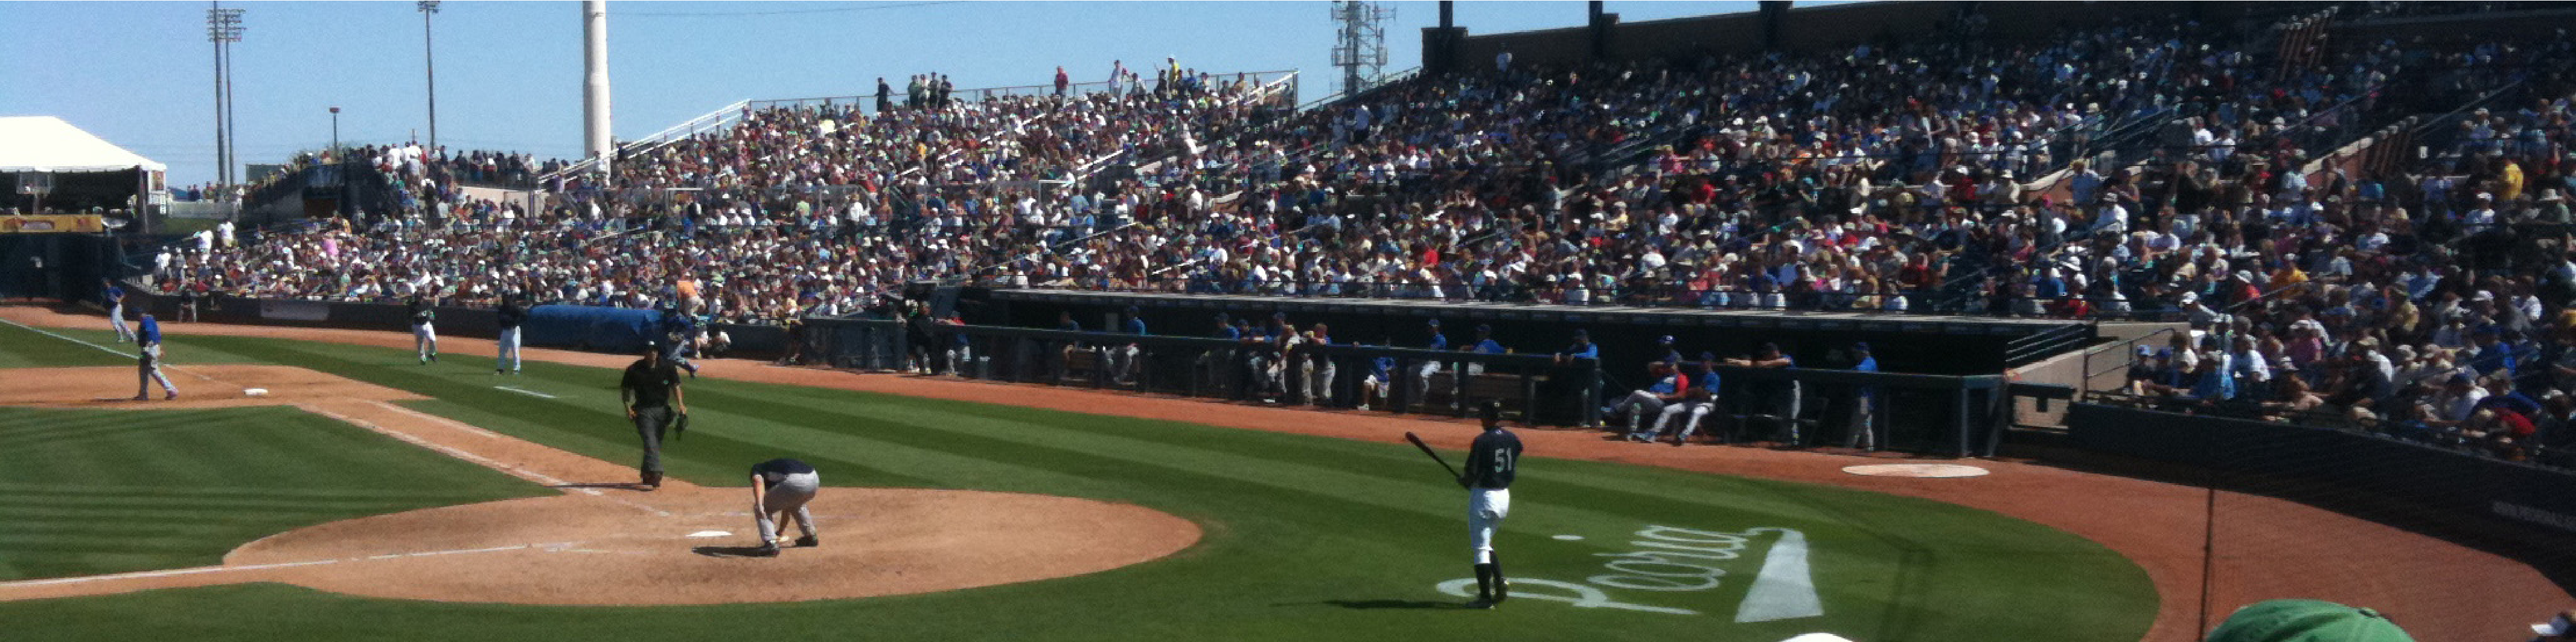
\includegraphics[height=1.5in]{images/sampleteaser}
%%   \caption{Spring Training 2009, Peoria, AZ.}
%% }

\maketitle

\begin{abstract}

Performance of interactive graphics walkthrough systems depend on the time taken to fetch the required data to render from the secondary storage to the main memory. It has been earlier established that a large fraction of this fetch time is spent on seeking the data on the hard disk. In order to reduce this seek time, redundant data storage has been proposed in the literature, but the redundancy factors of those layouts are prohibitively high.  In this paper, we develop a model for the seek time of a layout, and using this cost model, we propose an algorithm that would compute a redundant data layout with the redundancy factor that is within the user specified bounds while maximizing the performance of the system.



\end{abstract}

\begin{CRcatlist}
  \CRcat{I.3.6}{Computer Graphics}{Methodology and Techniques}{Graphics data structures and data types};
\end{CRcatlist}

\keywordlist

%% Use this only if you're preparing a technical paper to be published in the 
%% ACM 'Transactions on Graphics' journal.

\TOGlinkslist

%% Required for all content. 

\copyrightspace

\section{Introduction}

\subsection{Walkthrough Rendering}

In typical walkthrough systems, data sets consisting of hundreds of millions of triangles and many gigabytes of associated data are quite common. Rendering such massive amounts of data requires out-of-core rendering algorithms that bring only the required data for rendering into main memory from secondary storage. In this process, in addition to the rendering speed, the data fetch speed also becomes critical for interactivity. Data fetch speed depends on data seek time and data transfer time. Transfer time depends only on the amount of data that is transferred. Seek time is the time taken to locate the beginning of the required data in the storage device and depends on different things depending on the storage medium. \\
\\
For a hard disk drive (HDD), this seek time depends on the speed of the disk, and the relative placement of the data units with respect to each other, also called the data layout. For a solid state drive (SSD), this seek time is usually a small constant and is independent of the location of the data with respect to each other. Because of this, \cite{ssdpaper} showed that for SSDs, cache-coherent instead of cache-oblivious data layout is enough to reduce the total data fetch time and improve cache utilization. However, SSDs have many technical problems, including limited number of data overwrites allowed, high cost, and limited capacity.  \\
\\
On the other hand, the HDD  technology (including disk technologies such as CDs, DVDs, and Blu-ray discs) has become quite reliable and inexpensive and is thus in quite widespread use. Because of this, for massive data sets hard disk drives (HDD) are still and will be the preferred medium of storage for the foreseeable future. This means that addressing the seek time bottleneck in HDDs remains critical for interactive rendering. In this paper, we leverage the inexpensive nature of HDDs to store redundant copies of data in order to reduce the seek time. 

\subsection{Redundancy based data layouts}

Redundancy based data layouts to reduce the seek time were introduced in \cite{singleseeklayout}, in which the seek time for every access was reduced to at most one. However, in order to achieve this, the redundancy factor, the ratio between the size of the data after using redundancy to the original size of the data, was prohibitively high at around 80. In \cite{optimizingredundancy} the same authors related transfer volume, which dictates the data transfer time, seek time, and redundancy, and proposed a linear programming approach to optimize the data transfer and seek time in order to satisfy the total data fetch time constraint. In the process, redundancy was a hidden variable that was minimized. However, this procedure has many drawbacks.\\
\\
First, it provides a grouping of data units for each seek but it does not provide a data layout. This is because it does not relate one data group with another and it does not consider their relative layout. This could easily result in unnecessary data block duplications. The redundancy minimization is thus not modeled after physical representation of the data layout on the disk. The second major drawback is that the model for seek time is also not based on physical reality. Typically, seek time depends on the relative distance on the disk between the last data unit accessed and the data unit currently being requested. However, in \cite{optimizingredundancy}, seek time is simplistically modeled as number of seeks. This means that even if the requested data blocks are adjacent to each other and have no separate seek time to go from one block to another, this model would add them to the cost because it counts individual data blocks as one seek. 

\subsection{Main Contributions}

In this paper, we propose a model for seek time based on the actual distance between the data blocks in the linear data layout. Using this model, and given the spatial proximity of the data set for a walkthrough application, we develop an algorithm to duplicate data blocks strategically to maximize the reduction in the seek time while keeping the redundancy factor within the user defined bound. Note that an optimum data layout with redundancy that gives minimum seek time and redundancy factor is an NP-hard problem. However, we will show that our greedy solution generates both the extreme cases of data layout with redundancy, no redundancy (a simple cache oblivious mesh layout with low number of seeks) and maximum redundancy (a layout where seek time is at most one), as well as reasonable solutions for the redundancy factor constracts in between the extremes.


\section{Related Work}

Massive model rendering is a well studied problem in computer graphics. Most of the early works focused on increasing the rendering efficiency. At that time the fundamental problem was not fitting the model into the main memory but the speed of the graphics cards. Hence these works provided solutions to reduce the number of primitives to be rendered while maintaining the visual fidelity. These solutions included level-of-detail for geometric models \cite{Luebke}, progressive level of detail \cite{Hoppe, Garland}, and image based simplification \cite{Aliaga, HansongZhang}. Soon thereafter the size of the main memory became the bottleneck in handling ever increasing sizes of the model. Hence memory-less simplification techniques \cite{Lindstrom}  and other out-of-core rendering systems \cite{Correa, Varadhan} emerged in which just the limited amount of required data that needs to be processed and rendered was brought from the secondary storage to the main memory. \\
\\
Soon afterward, the researchers realized that the speed at which this data could be brought from the secondary to the main memory in these out-of-core algorithms is limited by the data bus speed, disk seek time, and data transfer time. They realized that these issues could be ameliorated to some extent by better cache utilization that would increase the utilization of data that is brought to the main memory and thus reduce the number of times the disk read is initiated. This meant that subsequent works focused on cache aware \cite{ssdpaper} and cache oblivious data layouts \cite{Yoon, other lindstrom's works} on the disk to reduce the  data fetch bottleneck. Our work falls under this class of algorithms that reduces the data fetch time. \\

\section{Greedy Redundancy-based Cache Oblivious Data Layout Algorithm}

For the purposes of this paper, we are given uniform data units in a linear sequence and each data unit has one or more access requirements assigned to it. An individual data units consists of geometric primitive data or other information that must be retrieved during walkthrough rendering. The access requirements are determined by the application and represent data units that will be accessed together during rendering. An example of this could be vertices that are spatially near each other. \\
\\
For an access requirement $A$, the total span of $A$ is the total number of data units between the first and last data units that use $A$. If a data unit does not use $A$ but lies between the first and last unit that does use $A$ then it is still counted in the span of $A$. Figure \ref{singleAR} shows a set of data units and explicitly labels the blue access requirement in this set. The total number of data units between the first and last blue unit is 14 thus that is the total length of the blue access requirement.\\
\\
\begin{figure}[ht]
\centering
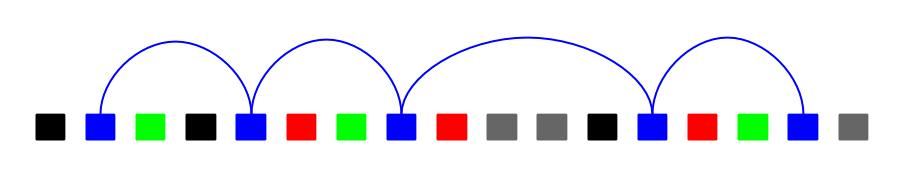
\includegraphics[width=3in]{SingleAR_start.jpg}
\caption{Illustration of a single access requirement}
\label{singleAR}
\end{figure}
Instead of trying to find the seek time explicitly while running, we use this layout to compute a probabilistic estimate for the seek time. Yoon's metric used the data layout to compute the expected number of times the cache would be missed, hence the number of times you would have to seek data from the hard disk. We extend this idea by thinking of an individual cache miss as an individual seek. We then assert that the Expected Seek Time (EST) is the total number of individual seeks that could be required. Because data units in an access requirement will be accessed together, the total number of seeks is the sum of the spans of all the access requirements. This is equivalent to Expected Cache Misses (ECM) in Yoon's paper. \\
\\
In that paper, Yoon is only allowed to move the data units around. His algorithm computes a locally optimal solution to minimizing ECM using only the move operation. In this paper, we are allowed to copy data units, move them, and delete old copies of data units. We want to figure out how to minimize EST while keeping the number of extra copies as low as possible. After running Yoon's algorithm to get an initial optimization, we take a data unit and copy it to a place that will mean shortening at least one of the access requirements that is attached to it. If the new data unit shortens all the access requirements attached to it, then we delete the old data unit. We repeat the individual copying and possible deletion procedure until our redundancy limit has been reached. \\
\\
{\bf Movable blocks:} Note that the cost of access does not change by moving an interior block to another interior location as the total length of the access requirement remains the same. Cost can be reduced only by moving the blocks that are at the either ends of the access requirement.This will greatly reduce the search space of data units to consider for copying. \\
\\
For the sake of simplicity of the algorithm, we operate on only one data block at a time. Based on the above argument, given an access requirement, we can possibly move the beginning or the end data block of the access requirement to the interior and make it an interior block. This will reduce the total span. In order to maximize our benefit to our current access requirement, we want to copy the start data unit to somewhere between the one after the first one and the last one. In the same manner, if the end data unit is better, we want to copy it to somewhere between the first one and the one before the last one. \\
\\
Figure \ref{singleARafterCopy} shows the access requirement from the above figure with an arrow showing the locations where the start unit can be moved to. By moving it to one of the these lcoations we are guaranteed to reduce the seek time for the access requirement. Figure \ref{singleARafterCopy2} shows the blue access requirement after the start unit has been copied. The dashed line connects the original data unit with its copy. The solid blue lines represent the new total span of the blue access requirement. The span of the blue access requirement has been reduced from 14 units in figure \ref{singleARafterCopy} to 12 units in figure \ref{singleARafterCopy2}.\\
\begin{figure}[ht]
\centering
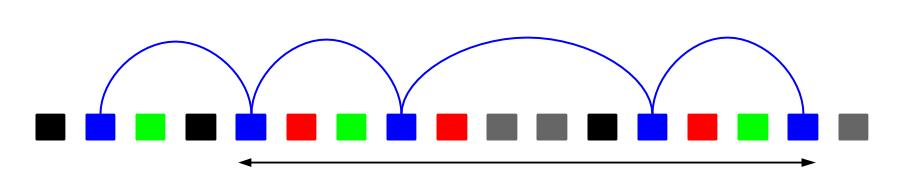
\includegraphics[width=3in]{SingleAR_afterCopy1.jpg}
\caption{Interval where the start data unit can be copied to}
\label{singleARafterCopy}
\end{figure}
\begin{figure}[ht]
\centering
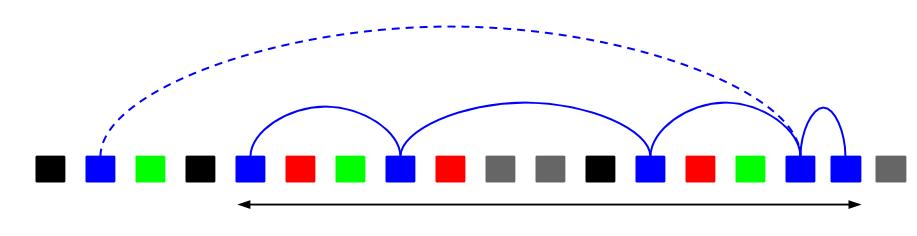
\includegraphics[width=3in]{SingleAR_afterCopy2.jpg}
\caption{Data units after the copying}
\label{singleARafterCopy2}
\end{figure}
\\
For the access requirement under consideration, it would not matter where in that interval we move the extremal data unit to. However, if the new location of the data block is in the span of other access requirements, it may increase the seek time of those accesses by one unit. Figure \ref{singleARafterCopyOtherAR} shows the above situation before the copying and highlights the gray access requirement that will be affected. As can be observed in figure \ref{singleARafterCopy2OtherAR} the gray access requirement has had its span increased by 1. Even though we reduced the total span by 2 with the blue access requirement, we also increased the total span by 1 with the gray access requirement, yield a net benefit of 1 data unit. We thus want to find a location that in the interior of the access requirement under consideration but is in the span of least number of access requirements. Such a location is identified using a simple linear search through the span of the access requirement.\\

\begin{figure}[ht]
\centering
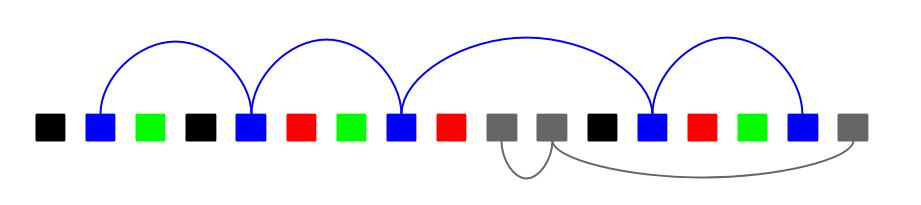
\includegraphics[width=3in]{SingleAR_afterCopy1_otherARnoted.jpg}
\caption{The blue and gray access requirements}
\label{singleARafterCopyOtherAR}
\end{figure}

\begin{figure}[ht]
\centering
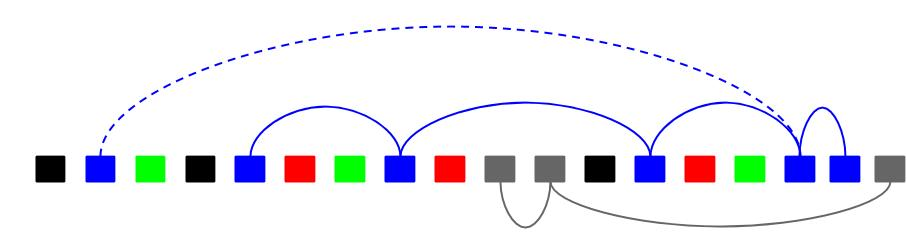
\includegraphics[width=3in]{SingleAR_afterCopy2_otherARnoted.jpg}
\caption{The blue and gray access requirements after the copy}
\label{singleARafterCopy2OtherAR}
\end{figure}

{\bf Moving versus Copying:} A data block can be accessed by multiple access requirements. If that data block is an extremal block of access, and if it is moved to its interior, it may affect other access requirements that use the same data block. That is the main reason that we are copying and not moving these data blocks. By copying the data unit the other access requirements can still access it in its old location without any change in their span. Nevertheless, if by using the new copy the span of one or more of the other access requirements reduces, then those access requirements should use the new copy instead of the old copy.\\
\\
{\bf  Deletion of a data block:} If all the access requirements use the new copy and the old data block is not used by any access, then it can be deleted.\\
\\
{\bf Data Block processing order:} We now need to figure out how to use this information to decide in what order the copying should be done. For each data unit, its total benefit is the amount that is reduces the total seek time ($EST$). For a given data unit to be copied to a specified location, let $k_i$ be the benefit to access requirement $i$ that is attached to the data unit. We will say that $k_i=0$ if the access requirement will use the old copy and $k_i>0$ if the access requirement will use the new copy. Let $I$ be the set of access requirements attached to the data unit. Finally, let $M$ be the number of overlapping access requirements at the location chosen. We can now describe the benefit as follows:
\[
Benefit = -\Delta EST = \sum_{i \in I} k_i - M
\]
Before doing any actual copying, we compute the above described benefit for each start and end data unit for each access requirement. We store all the benefits into a binary search tree sorted in descending order by benefit amount. That way we will easily be able to choose the data unit that provides the most benefit in expected seek time. We will also make a special list $L$ of cases where a data unit is copied then deleted because all the access requirements will benefit. \\
\\
Because doing the copying in $L$ does not increase the storage, we will first go through that list and do the copying. Once that list is empty we will take the data unit in the binary search tree that provides the most benefit and perform the copy. We will then recompute $L$ and the binary search tree. We will continue to do those steps until we have run out of available space for redundancy.  

\subsection{Algorithm Summary}

\begin{verbatim}

AR: access requirement

Initialize AR heap and newCopy list
for each AR P's head node and tail node U:
     Let S = next or previous node
     Set BENEFIT=distance(S,U)
     Let copy of U be U'
     Put U' in place between S and U with:
          least number of overlapping ARs
     For each AR T that also uses U
          If T will be shorter by U':
               Add T's benefit to BENEFIT
          Else:
               Add T to oldCopyList
     Add BENEFIT to heap
     If oldCopyList is empty:
          add U to newCopy list
while newCopy is not empty:
     take out random element and move the node
     Update AR heap and newCopy list
while there exists more space for redundancy:
     pop best element from heap
     copy the element U to its destination
     update affected access requirements
     update heap

\end{verbatim}

\section{Run-time and Storage Analysis}

We now need to analyze the running time and storage requirements of our algorithm. We will denote $N$ as the number of data units and $A$ as the number of access requirements. We will use $k$ as the average length of a single access requirement. The variable $Q$ will represent the number of runs of the redundancy and new copy loop. The average number of overlapping access requirements is proportional to the number of data units multiplied by the redundancy factor $r$, which is the amount of redundancy if we have a single-seek layout. Therefore, the number of overlapping access requirements is O(rN). 

\subsection{Run-time Analysis}

The Initial Construction loop is run on all A access requirements. It involves finding all the benefit information and putting it into a heap so that it is easy to figure out the best access requirement to modify first. There are log(A) operations to insert the data into the heap and a constant number of operations plus O(k) operations for the search of the AR to get the benefit information. Thus it takes a total of $O(A \cdot k \cdot logA)$ operations to do the initial construction. \\
\\
With the new copy and redundancy loops, there are O(rN) overlapping access requirements and a constant number of operations for each access requirement. Then, the algorithm reforms the heap and updates the nodes in the AR. With that, there are $O(log(A))$ operations done a constant number of times plus O(k) operations for updating the data nodes in the access requirement. Thus the redundancy and new copy loop takes $O(Q(k \cdot logA + rN))$ operations. \\
\\
This means that in total, our algorithm takes $O( k \cdot logA (Q+A) + rN)$ operations. 

\subsection{Storage Analysis}

During the run of the algorithm, we have to store the number of overlapping access requirements at each data unit, which will require $O(N)$ storage. We will also have to store a heap of access requirements, which can be stored using $O(A)$ space. We also have a list of access requirements and that information will take up $O(A)$ space. In total we thus have $O(A + N)$ storage space used during the run of the algorithm. 


\subsection{Linear search justification}

Here I justify why we do a simple linear search in the part of the algorithm where we decide where to put the new data unit. The original problem is to find the least number in an arbitrary block of a list. If $k$ is the size of the access requirement, then this gives us $O(k)$ query time. Updates will also be $O(k)$ and construction will be $O(N)$ with N being the number of data units. There are other approaches, such as a range tree or dynamic programming, that may produce better query times, but their construction and update times will be worse as well as their storage. \\
\\
With dynamic programming, we would have to maintain a matrix where an entry $(i,j)$ would contain the minimum value in that range. This would give us a $O(1)$ query time but the construction and storage would be $O(N^2)$ where N is the number of data units. The update time would be $O(N)$ when we add a data unit. Since the $N$ for this problem domain is in the hundreds of millions, that is an unacceptable storage bound. The construction run time would also be prohibitive given the magnitude of our input. \\
\\
We could use a range tree. The initial binary search tree would be sorted by index and at each entry would be a pointer to a binary search tree sorted by value. If we put the min value at each of the nodes of the initial tree, we can speed up our queries. We would get a $O(log N)$ query time, but our construction time and storage would be $O(N log N)$. Updating the data structure would take at a minimum $O(k log(N))$ time if we do careful indexing and only update the nodes that need to be updated. If we have a large access requirement, then this would represent a significant improvement in query time however given our exceptionally large input, the construction, storage, and update bounds are too prohibitive.  


\section{Theoretical Improvements over existing algorithms}

The initial part of the algorithm where we copy and delete units will produce a better solution than proposed by Yoon without adding extra units. This is because our algorithm will consider cases where data units are close to each other but in different blocks of units that would be arranged in Yoon's algorithm. Consider a case where we have two access requirements of 5 data units each. Figure \ref{YoonImprovement1} shows an example of that. Figure \ref{YoonImprovement2} shows the result of using Yoon's algorithm. Because its hierarchical it would arrange the units in each block and then arrange the blocks. Thus even though the black access requirement blocks can be grouped together, Yoon's heuristic would not detect that. When our algorithm is run after Yoon's algorithm, it would find that it can shorten the black access requirements without adding redundancy so it would do that first. You would end up with the ideal solution as shown in figure \ref{YoonImprovement3}

\begin{figure}[ht]
\centering
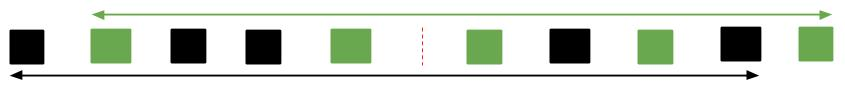
\includegraphics[width=3in]{ImprovementOverYoon_before.jpg}
\caption{Example of two access requirements of 5 data units each. The red line represents the boundary between blocks that Yoon's algorithm would use}
\label{YoonImprovement1}
\end{figure}

\begin{figure}[ht]
\centering
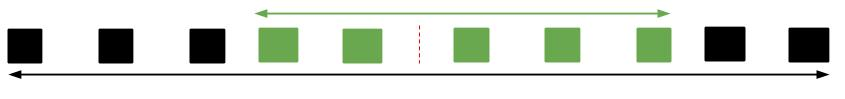
\includegraphics[width=3in]{ImprovementOverYoon_afterYoons.jpg}
\caption{The above figure after running Yoon's algorithm}
\label{YoonImprovement2}
\end{figure}

\begin{figure}[ht]
\centering
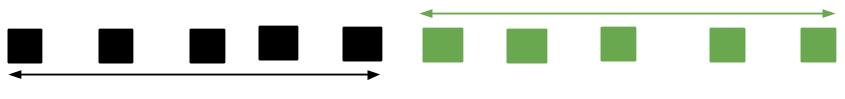
\includegraphics[width=3in]{ImprovementOverYoon_afterOurs.jpg}
\caption{The above figure after running our algorithm}
\label{YoonImprovement3}
\end{figure}

Existing algorithms for the data layout problem do not consider redundancy. Even if we find a polynomial solution to the data layout problem, we can actually achieve a seek time better than the optimal one without redundancy. Figure \ref{fig:startingProb} shows a case where that happens. The total seek time is 11 units. Without redundancy, the optimal solution is shown in Figure \ref{woRedundacy}. The seek time has been reduced to 9 units. With redundancy, the total seek time is now the minimum required which is 7 units, as shown in Figure \ref{withRedundancy}. While a reduction from 9 to 7 units may not seem dramatic, when this result is scaled up to the hundreds of millions, this makes a big difference in seek time, which we saw in practice as described in the next section.\\

\begin{figure}[ht]
\centering
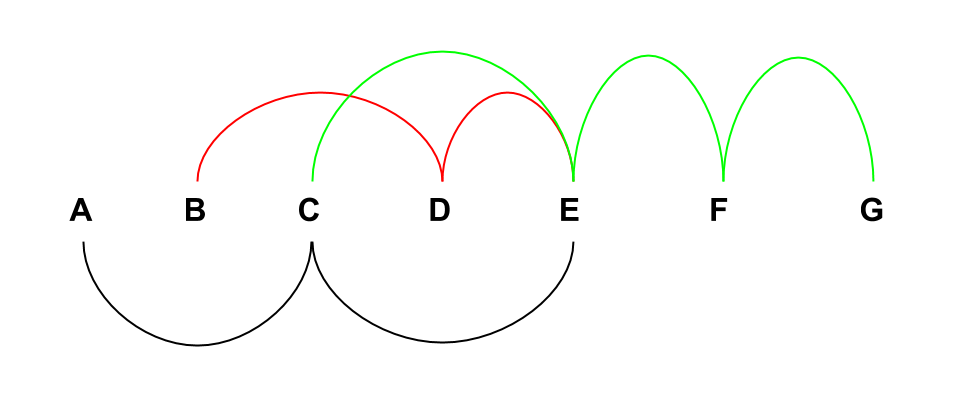
\includegraphics[width=3in]{examplePic_startingProblem.png}
\caption{Data Units with varying access requirements}
\label{fig:startingProb}
\end{figure}

\begin{figure}[ht]
\centering
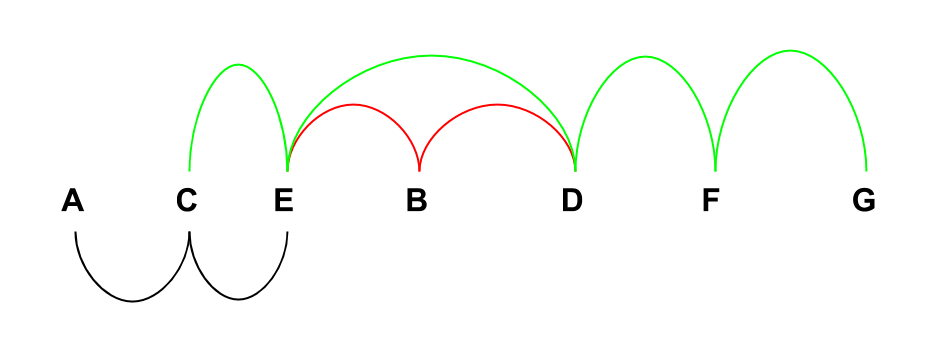
\includegraphics[width=3in]{examplePic_woRedundancy.png}
\label{woRedundacy}
\caption{Optimal layout without redundancy}
\end{figure}

\begin{figure}[ht]
\centering
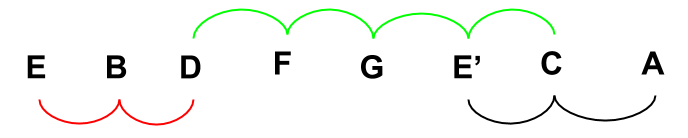
\includegraphics[width=3in]{examplePic_withRedundancy.png}
\label{withRedundancy}
\caption{Optimal layout with redundancy. The data unit E' is the redundant copy of E.}
\end{figure} 

\section{Experimental Results}

\begin{figure}[ht]
  \centering
  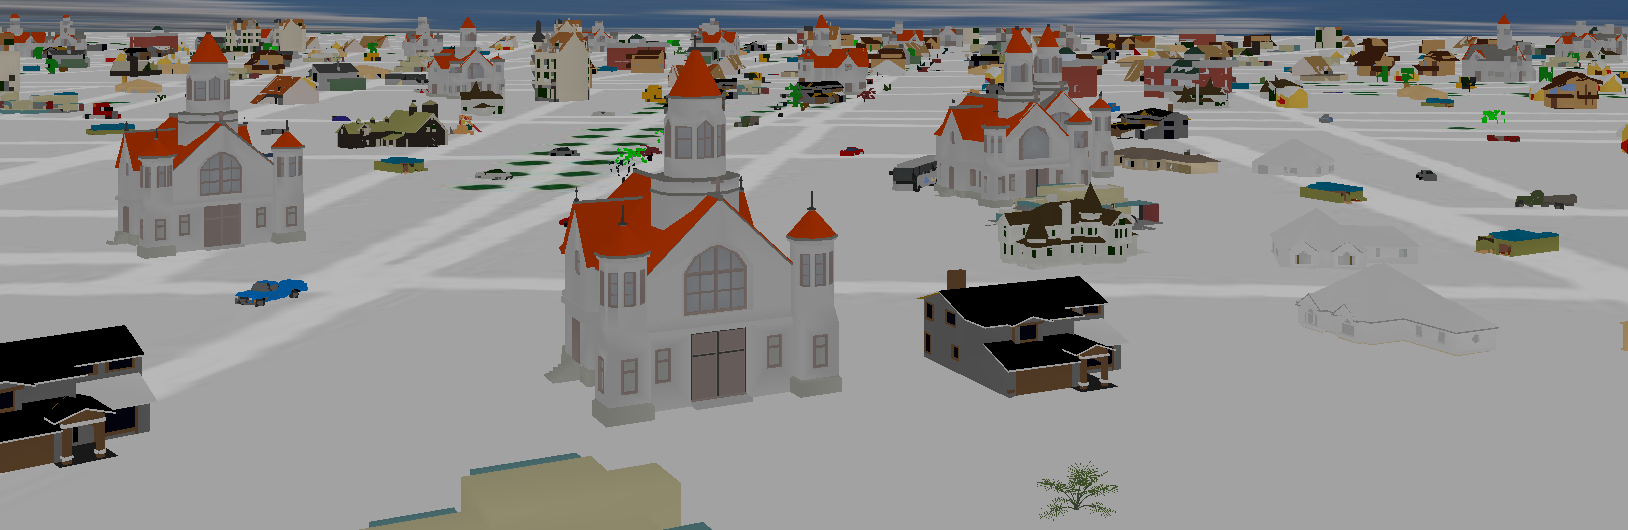
\includegraphics[width=3.0in]{city.png}
  \caption{City model: 110 million triangle, 6 GBs. }
  \label{fig:model1}
\end{figure}

\begin{figure}[ht]
  \centering
  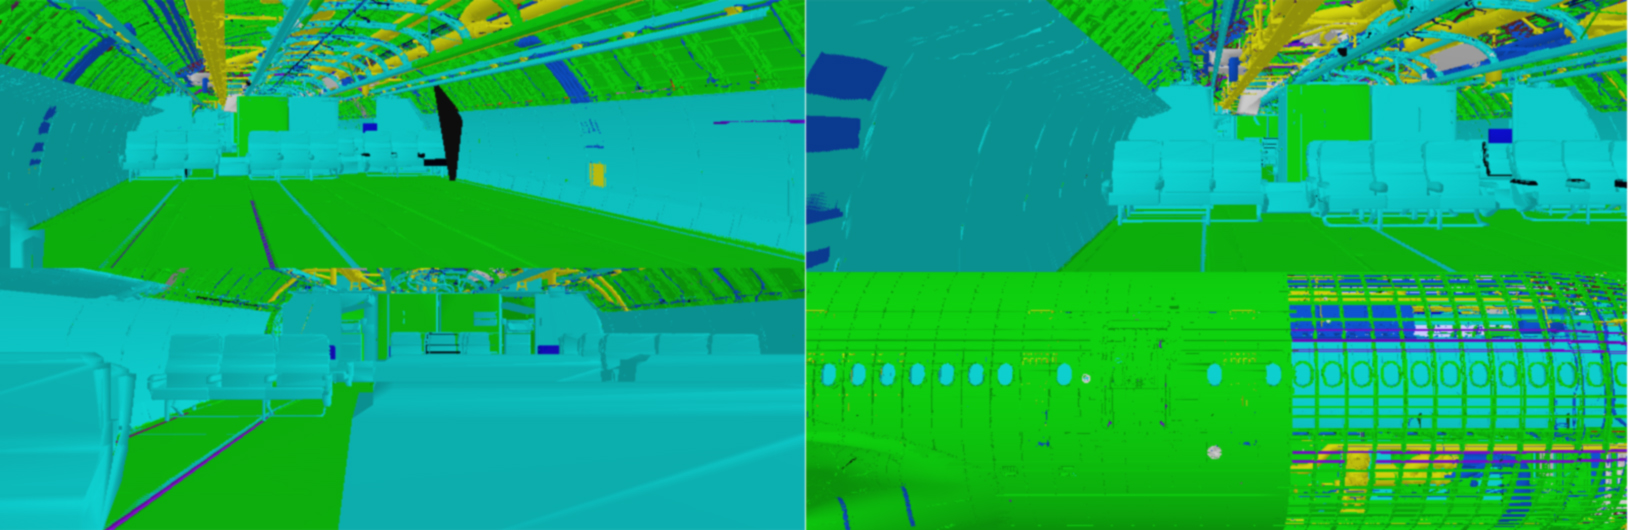
\includegraphics[width=3.0in]{boeing.jpg}
  \caption{Boeing model: 350 million triangle, 20 GBs. }
  \label{fig:model2}
\end{figure}

\begin{figure}[ht]
  \centering
  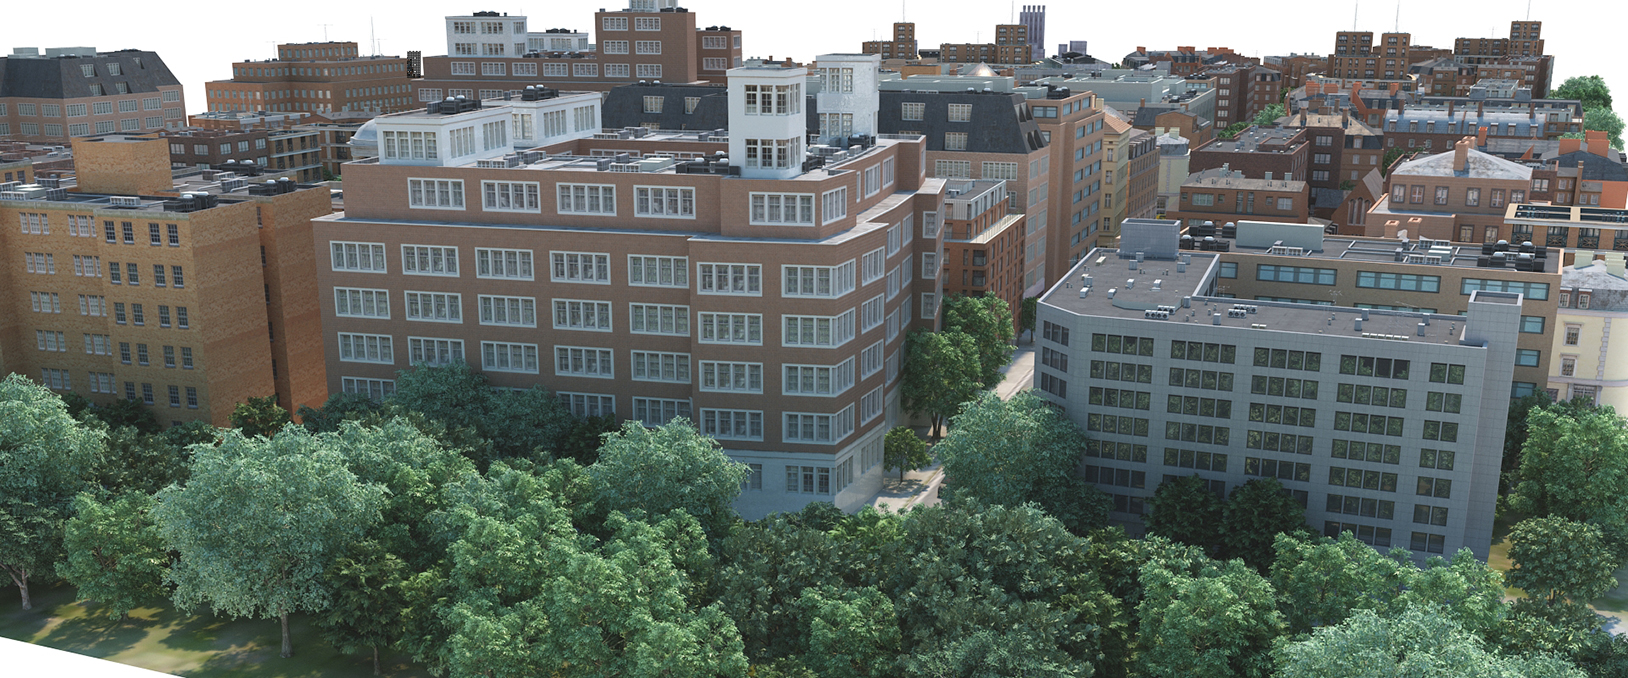
\includegraphics[width=3.0in]{densecity.jpg}
  \caption{Urban model: 100 million triangle, 12 GBs. }
  \label{fig:model3}
\end{figure}


\textbf{Experiment context:}
In order to implement our algorithm, we used a workstation that is a Dell T5400 PC with Intel (R) Core (TM) 2 Quad and $8GB$ main memory. The hard drive is a 1TB Seagate Barracuda with 7200 RPM and the graphics card is an nVIDIA Geforce GTX 260 with 896 MB GPU memory. The data rate of the hard drive is $120$ MB/s and the seek time is a minimum of $2$ ms per disk seek.\\
\\
\textbf{Benchmarks:}
We use three models to perform our experiments, each model represents a use case or scenario. The City model (Figure \ref{fig:model1}) is a regular model might be used in a navigation simulation application or visual reality walkthough. The Boeing model (Figure \ref{fig:model2}), on the other hand, represents scientific or engineering visualization applications. The Urban model has texture attached to it, which is commonly used in games. By comparing performance of cache-oblivious layout without redundancy and with redundancy on these three models, our goal is to show the redundancy based approach can achieve more stable and generally better performance on different real time applications. \\
\\
\textbf{Results:}
Figure \ref{fig:resultall} shows the results of delays caused by fetching data on the experimental models we used. We compare the results of a cache-oblivious layout without redundancy and one with redundancy. For the layout with redundancy, we set the redundancy factor equal to 4.2. It is clear that the performance of the layout with redundancy has generally shorter delays than the cache-oblivious layout without redundancy. As can be observed from the results, although the layout with redundancy does not eliminate delays for most of sample points on the walkthrough path, it reduces delays to a small range and keeps the performance more consistent. This is the benefit we get from using our algorithm which adds redundancy. Since the algorithm tends to eliminate seeks with longer seek time first, in practice the larger delays are avoided.\\
\\

\begin{figure}[ht]
\centering
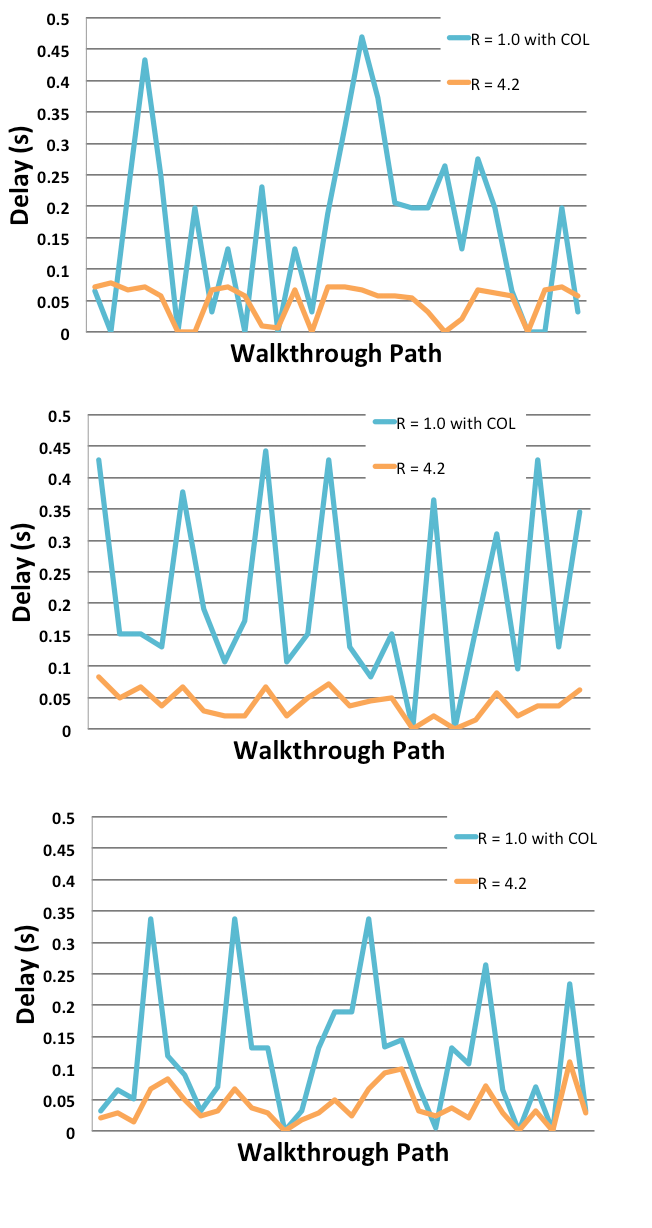
\includegraphics[width=3.0in]
{resultall.png}
  \caption{Statistics of delays caused by the fetching processes for the Sparse City model (top), the Boeing model (center), and
the Dense City model (bottom), with and without redundancy. }
  \label{fig:resultall}
\end{figure} 

\begin{figure}[ht]
\centering
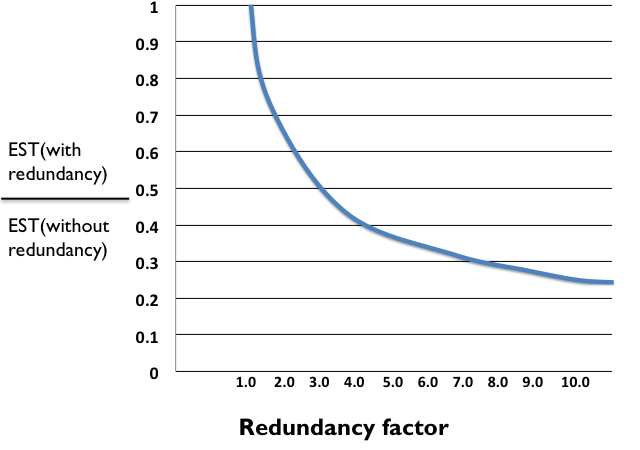
\includegraphics[width=3.0in]{statistic.png}
  \caption{Plot of the ratio of the EST of layout with redundancy over the EST of cache-oblivious mesh layout withou redundancy. }
  \label{fig:statistic}
\end{figure} 

There is another major benefit to our approach. Since each time we duplicate one data unit, we can halt it when the redundancy factor reaches a certain threshold. This helps us create a data layout with arbitrary redundancy factor without worrying about exceeding the capacity of secondary storage devices. We use this fact to test different redundancy factors and see their results. In Figure \ref{fig:statistic}, we show the results of using layouts with redundancy factors that range from 1.0 to 10.0. The y-axis in this figure is the ratio of the estimated seek time (EST) of the layout with redundancy over the EST of the layout without redundancy. This value starts at 1.0 where redundancy factor is 1.0, meaning no redundancy, and decreases as redundancy factor goes larger. We can see that the rate of this decrement is not constant, and the benefits we gain at beginning are larger than the ones we get later. This implies that most of the performance improvement resides at the earlier phase of raising redundancy factor. This implies that it is worth it to limit the redundancy factor used because after a certain point you are using much more secondary storage space without improving seek time by much. It also implies that our algorithm dramatically reduces seek time in practice by using only small redundancy factors. \\  
\\


\section{Conclusion and Future Work}

We have shown that we have an algorithm with an efficient running time and storage space for the Data Layout Problem. It achieves significant results analytically and experimentally. When walking through an extremely detailed 3D model, this algorithm can be used to ensure that the performance will not suffer. If we give the algorithm the proper access requirements with this 3D model, then the performance will be even better.\\
\\
This leads to a logical extension of this work. Since we have a good algorithm that takes over once we know the access requirements, we should figure out how to ensure there are good access requirements to begin with. One idea on how to ensure this is to check the usage history of an application and group data units together if they are accessed together with high probability. This could even be done dynamically in the sense that after a certain amount of usage and repeating on a regular basis, you recompute the optimal access requirements and then use that to recompute the optimal layout. 

\bibliographystyle{acmsiggraph}
\bibliography{finalPaperRefs}

\end{document}
